\documentclass[UTF8,a4paper,12pt]{ctexbook} 

\usepackage{graphicx}%学习插入图
\usepackage{verbatim}%学习注释多行
\usepackage{booktabs}%表格
\usepackage{geometry}%图片
\usepackage{amsmath}
\usepackage{amssymb}
\usepackage{listings}%代码
\usepackage{xcolor}  %颜色
\usepackage{enumitem}%列表格式
\setenumerate[1]{itemsep=0pt,partopsep=0pt,parsep=\parskip,topsep=5pt}
\setitemize[1]{itemsep=0pt,partopsep=0pt,parsep=\parskip,topsep=5pt}
\setdescription{itemsep=0pt,partopsep=0pt,parsep=\parskip,topsep=5pt}
\usepackage{tcolorbox}
\usepackage{algorithm}  %format of the algorithm
\usepackage{algorithmic}%format of the algorithm
\usepackage{multirow}   %multirow for format of table
\usepackage{tabularx} 	%表格排版格式控制
\usepackage{array}	%表格排版格式控制
\usepackage{hyperref} %超链接 \url{URL}
\usepackage{tikz}
\usepackage{dirtree}


\usetikzlibrary{intersections,
	positioning,
	petri,
	backgrounds,
	fit,
	decorations.pathmorphing,
	arrows,
	arrows.meta,
	bending,
	calc,
	intersections,
	through,
	backgrounds,
	shapes.geometric,
	quotes,
	matrix,
	trees,
	shapes.symbols,
	graphs,
	math,
	patterns,
	external}
\CTEXsetup[format+={\flushleft}]{section}

%%%% 设置图片目录
\graphicspath{{figure/}}

%%%% 段落首行缩进两个字 %%%%
\makeatletter
\let\@afterindentfalse\@afterindenttrue
\@afterindenttrue
\makeatother
\setlength{\parindent}{2em}  %中文缩进两个汉字位

%%%% 下面的命令重定义页面边距,使其符合中文刊物习惯 %%%%
\addtolength{\topmargin}{-54pt}
\setlength{\oddsidemargin}{0.63cm}  % 3.17cm - 1 inch
\setlength{\evensidemargin}{\oddsidemargin}
\setlength{\textwidth}{14.66cm}
\setlength{\textheight}{24.00cm}    % 24.62

%%%% 下面的命令设置行间距与段落间距 %%%%
\linespread{1.4}
\setlength{\parskip}{0.5\baselineskip}
\geometry{left=1.6cm,right=1.8cm,top=2cm,bottom=1.7cm} %设置文章宽度
\pagestyle{plain} 		  %设置页面布局

%代码效果定义
\definecolor{mygreen}{rgb}{0,0.6,0}
\definecolor{mygray}{rgb}{0.5,0.5,0.5}
\definecolor{mymauve}{rgb}{0.58,0,0.82}
\lstset{ %
	backgroundcolor=\color{white},   % choose the background color
	basicstyle=\footnotesize\ttfamily,      % size of fonts used for the code
	%stringstyle=\color{codepurple},
	%basicstyle=\footnotesize,
	%breakatwhitespace=false,         
	%breaklines=true,                 
	%captionpos=b,                    
	%keepspaces=true,                 
	%numbers=left,                    
	%numbersep=5pt,                  
	%showspaces=false,                
	%showstringspaces=false,
	%showtabs=false,        
	columns=fullflexible,
	breaklines=true,                 % automatic line breaking only at whitespace
	captionpos=b,                    % sets the caption-position to bottom
	tabsize=4,
	commentstyle=\color{mygreen},    % comment style
	escapeinside={\%*}{*)},          % if you want to add LaTeX within your code
	keywordstyle=\color{blue},       % keyword style
	stringstyle=\color{mymauve}\ttfamily,     % string literal style
	frame=L,
	xleftmargin = .06\textwidth,
	rulesepcolor=\color{red!20!green!20!blue!20},
	% identifierstyle=\color{red},
	language=php,
}
 \author{\kaishu 郑华}
 \title{\heiti PHP 学习笔记}
 
\begin{document}          %正文排版开始
 	\maketitle
 	\tableofcontents

\chapter{PHP 简介}	
 	\url{http://php.net/manual/zh/}
 	\section{用途}
 		PHP 脚本主要用于以下三个领域:
 		
 		\begin{itemize}
 			\item \textbf{服务端脚本}。这是 PHP 最传统,也是最主要的目标领域。开展这项工作\textbf{需要具备以下三点}:
 				\begin{enumerate}
 					\item PHP 解析器(\verb|CGI| 或者 \verb|服务器模块|)
 					\item Web 服务器
 					\item Web 浏览器
 				\end{enumerate}
 			需要在运行 web 服务器时,安装并配置 PHP,然后,可以用 web 浏览器来访问 PHP 程序的输出,即浏览服务端的 PHP 页面。如果只是实验 PHP 编程,所有的这些都可以运行在自己家里的电脑中。
 			
 			\item \textbf{命令行脚本}。可以编写一段 PHP 脚本,并且不需要任何服务器或者浏览器来运行它。通过这种方式,仅仅只需要 PHP 解析器来执行。这种用法对于依赖 cron(Unix 或者 Linux 环境)或者 Task Scheduler(Windows 环境)的日常运行的脚本来说是理想的选择。这些脚本也可以用来处理简单的文本。
 			
 			\item \textbf{编写桌面应用程序}。对于有着图形界面的桌面应用程序来说,PHP 或许不是一种最好的语言,但是如果用户非常精通 PHP,并且希望在客户端应用程序中使用 PHP 的一些高级特性,可以利用 PHP-GTK 来编写这些程序。用这种方法,还可以编写跨平台的应用程序。PHP-GTK 是 PHP 的一个扩展,在通常发布的 PHP 包中并不包含它。
 		\end{itemize}
 		
 		
 		使用 PHP,并\textbf{不局限于输出 HTML}。PHP 还能被用来动态输出图像、PDF 文件甚至 Flash 动画(使用 libswf 和 Ming)。还能够非常简便的输出文本,例如 XHTML 以及任何其它形式的 XML 文件。PHP 能够自动生成这些文件,在服务端开辟出一块动态内容的缓存,可以直接把它们打印出来,或者将它们存储到文件系统中。
 		
 		PHP 最强大最显著的特性之一,是它支持很大范围的\textbf{数据库}。使用任何针对某数据库的扩展(例如 mysql)编写数据库支持的网页非常简单,或者使用抽象层如 PDO,或者通过 ODBC 扩展连接到任何支持 ODBC 标准的数据库。其它一些数据库也可能会用 cURL 或者 sockets,例如 CouchDB。
 		
 		PHP 还支持利用诸如 LDAP、IMAP、SNMP、NNTP、POP3、HTTP、COM(Windows 环境)等不计其数的\textbf{协议}的服务。还可以开放原始网络端口,使得任何其它的协议能够协同工作。PHP 支持和所有 web 开发语言之间的 WDDX 复杂数据交换。关于相互连接,PHP 已经支持了对 Java 对象的即时连接,并且可以透明地将其用作 PHP 对象。
 	
 	
 	\section{配置}
 		主要参考\url{https://www.cnblogs.com/cyrfr/p/6483529.html}
 		
 		开发参考\url{https://www.douban.com/group/topic/111428204/}
 		\subsection{Apache2.4}
 			\paragraph{简介}
 				\begin{itemize}
 					\item HTTP Server
 					\item 支持最新的HTTP/1.1 通信协议
 					\item 支持FastCGI
 					\item 支持多种方式的HTTP认证等
 				\end{itemize}
	 		\paragraph{httpd.conf}
	 			主要用于设置 Apache2 服务器的跟目录、PHP 模块关联。
	 			\begin{itemize}
	 				\item 服务器的根目录 
	 					\begin{lstlisting}
	 Define SRVROOT "D:/LAMP-AMP/APACHE_2.4/Apache24"
	 ServerRoot "${SRVROOT}"  // 指定守护进程httpd的运行目录
	 DocumentRoot "D:/Develop/Apache2.2/htdocs"  // 指定站点目录
	 <Directory "D:/Develop/Apache2.2/htdocs">   // 指定目录执行规则
	 
	 					\end{lstlisting}
	 					
	 				\item PHP 模块关联,包括模块库、访问类型、PHP主目录
	 					\begin{lstlisting}
	 LoadModule php7_module D:/LAMP-AMP/PHP_7.1/php7apache2_4.dll  
	 AddType application/x-httpd-php .php .html .htm
	 PHPIniDir D:/LAMP-AMP/PHP_7.1
	 					\end{lstlisting}
	 			\end{itemize}
	 			
	 			\subparagraph{ServerRoot}
	 				ServerRoot用于指定守护进程httpd的运行目录,httpd在启动之后将自动将进程的当前目录改变为这个目录,因此如果设置文件中指定的文件或目录是相对路径,那么真实路径就位于这个ServerRoot定义的路径之下。 
	 				
	 		\paragraph{启动 Apache 服务}	
	 			\begin{itemize}
	 				\item Windows
	 					\begin{itemize}
	 						\item 开启服务 \verb|net start mysql|
	 						\item 停止服务 \verb|net stop mysql|
	 						\item 移除服务 \verb|mysqld -remove|
	 					\end{itemize}
	 				\item Linux
	 					\verb|\etc\init.d\apache2 start|
	 			\end{itemize}
	 			
 		\subsection{php.ini}	
 			设置php 的时间 \verb|date.timezone = Asia/Shanghai|

 		\subsection{FastCGI}
 		 	To Be Continue...	
 		 		
\chapter{基本语法}
	\section{变量}
		
		\paragraph{变量}
			随身携带\verb|$|
			
			使用\textbf{其他文件变量}时,使用\verb|include 'fileName'|
		
		\paragraph{传值}
			就是单纯的将值赋值给形参,和copy是一样的
			
		\paragraph{传引用}
			类似于C++语言的引用
			
			\begin{lstlisting}
<?php    
	$param2=1;               //定义变量2    
	$param1 = &$param2;      //将变量2的引用传给变量1    
	echo $param2;            //显示为1    
	$param1 = 2;             //把2赋值给变量1    
	echo $param2;            //显示为2    
?> 
			\end{lstlisting}
			
	\section{作用域}
		\begin{itemize}
			\item 局部变量
			\item 全局变量:将所有全局变量存储在一个名为 \verb|$GLOBALS[index]| 的数组中。 \verb|index| 保存变量的名称。这个数组可以在函数内部访问,也可以直接用来更新全局变量。
			\item 静态变量:当一个函数完成时,它的所有变量通常都会被删除。然而,有时候您希望某个局部变量不要被删除。要做到这一点,请在您第一次声明变量时使用 \verb|static| 关键字
		\end{itemize}
	
		\paragraph{超级全局变量}
			\begin{itemize}
				\item \verb|$GLOBALS |是一个包含了\textbf{全部变量的全局组合数组}。变量的名字就是数组的键。
				\item \verb|$_SERVER |是一个包含了诸如头信息(header)、路径(path)、以及脚本位置(script locations)等等信息的数组。这个数组中的项目\textbf{由 Web 服务器创建}。不能保证每个服务器都提供全部项目;具体含义查看\url{http://www.runoob.com/php/php-superglobals.html}
				\item \verb|PHP $_REQUEST |用于收集HTML表单提交的数据。
				\item \verb|PHP $_POST |变量是一个数组,内容是由 HTTP POST 方法发送的变量名称和值。可以在网址的栏目上是\textbf{看不到}传送的内容的
				\item \verb|PHP $_GET |变量是一个数组,内容是由 HTTP GET 方法发送的变量名称和值。可以在网址的栏目是\textbf{看到}内容的
			\end{itemize}
		
		\paragraph{花括号的区别}
			很多语言都以花括号作为作用域界限,PHP中只有函数的花括号才构成新的作用域。
			
			\url{https://www.cnblogs.com/52php/p/5670067.html}	
	\section{数组}
		\paragraph{形式}
			\begin{itemize}
				\item 普通数组:\verb|$cars = array("Volvo","BMW","Toyota");|
				\item 键值数组:\verb|$cars = array("Volvo"=>"30","BMW"=>"40","Toyota"=>"50");|
				\item 二维数组:
					\begin{lstlisting}
	$cars = array(
		array("volvo",100,96),
		array("bmw",99,34),
		array("toyota",33,24)
	);
					\end{lstlisting}
				\item 新写法:\verb|$cars= ["2","3","5"];|
				\item 初始化新方法:
					\begin{lstlisting}
	$arr = array(5 => 1, 12 => 2);
	
	$arr[] = 56;    // This is the same as $arr[13] = 56;
	                // at this point of the script
					\end{lstlisting}
			\end{itemize}
			
		
		\subsection{数组函数}
			\begin{itemize}
				\item \verb|count($arrVar) :统计数组变量个数|
				\item \verb|foreach($arrVar as $varElement)|
				\item \verb|foreach($arrKeyVar as $keyElement => $valueElement )|
				\item \verb|array_keys()| 返回数组中所有的键名
				\item \verb|array_pop()| 出栈
				\item \verb|array_push()| 入栈
				\item \verb|array_rand()| 随机选出一个或多个元素
				\item \verb|array_shift()| 删除数组中的第一个元素,并返回删除元素的值,出队
				\item \verb|in_array()| 检查数组中是否存在指定的值
			\end{itemize}	
			
	
	\section{字符串函数}
		\begin{itemize}
			\item \verb|explode()| 将字符串转化成数组
			\item \verb|implode()| 将数组合并成一个字符串,等价于\verb|join()|
			\item \verb|trim()| 去掉字符串两边的字符
			\item \verb|md5()| 计算字符串的md5散列
			\item \verb|str_replace()| 替换字符串中的一些字符。
		\end{itemize}		
	\section{面向对象}
		与c++  大致一致,需要注意一下特性。
		\begin{itemize}
			\item 对象变量\textbf{默认为指针},需要使用\verb|->|调用成员函数。
			\item \verb|$this| this 变量也不例外需要使用 \verb|$|, 与之对应的有\verb|self::成员变量 |
			\item 构造函数 \verb|function __construct($args)|
			\item 析构函数 \verb|function __destruct()|
			\item 继承 使用关键字\verb|extends |
			\item 接口 使用关键字\verb|interface、implements|类似于Java
			\item final 标识的方法,子类不能再对其覆盖重写
			\item PHP \textbf{不会}在子类的构造方法中\textbf{自动}的\textbf{调用父类的构造方法}。要执行父类的构造方法,需要在子类的构造方法中调用 \verb|parent::__construct()| , 同理,\textbf{使用父类方法}\verb|parent::xx()|
		\end{itemize}
		
	
	
	\section{表单原理}
		主要参考\url{https://www.cnblogs.com/qiujun/p/6801896.html}
		
		\subsection{form 表单}
			\begin{itemize}
				\item \verb|GET| \textbf{将表单内容附加到URL地址后面},提交的信息\textit{长度有限制},\textbf{不可以超过8192个字节},\textit{同时不具有保密性,而且只能传送ASCII字符}(一般传送的不保密性数据)
				\item \verb|POST| \textbf{将用户填写的数据包含在表单数据中},\textit{不会在地址栏中显示,同时没有数据长度的限制}
			\end{itemize}
			
			默认GET方法,地址传值使用的GET方法
			
		\subsection{input 标记}
			\begin{itemize}
				\item \verb|type| 属性
					\begin{itemize}
						\item \verb|text| 文本域
						\item \verb|password| 密码域
						\item \verb|radio| 单选框
						\item \verb|file| 文件等
					\end{itemize}
				\item \verb|name| 表单名称
				\item \verb|action| \textbf{目标地址},绝对或相对URL,默认为当前页面
				\item \verb|enctype| 表单编码方式
				\item \verb|$_POST| 数据存储于此处
			\end{itemize}
		
		\subsection{数据获取方式}
			\begin{itemize}
				\item \verb|$_GET['key']| || \verb|$_POST['key']|
				\item \verb|isset($variable)| :判断一个变量是否设置,isset判断变量是否已存在(配置)
				\item \verb|empty($variable)| :empty 判断变量是否为空
			\end{itemize}
			
			常用判断:\url{https://blog.csdn.net/qiangzaiying123/article/details/62068438}
	
	\section{JSON 读写}
		\subsection{JSON 基本格式}
			\begin{itemize}
				\item 数组:\verb|[1,2,4,"hello",[4,5,6], {"w":"World"}]|
				\item 对象:\verb|{"h":"Hello", "w":"World", [1,2,3]}|
			\end{itemize}
		
			\subparagraph{PHP 打印方式}
				\begin{itemize}
					\item 打印对象:\verb|print_r($obj)|
					\item 打印字符传:\verb|echo ""|
				\end{itemize}
			
		\subsection{encode}
			\verb|json_encode($obj)|
			
			\begin{lstlisting}
	$arr = array(1,2,3,'Hello','World',array('h'=>'Hello','w'=>'World'));
	echo json_encode($arr);
			\end{lstlisting}
		
		\subsection{decode}
			\verb|json_decode($obj)|
			
			\begin{lstlisting}
	$json_str = '{"h":"Hello", "w":"World"}';
	$obj = json_decode($json_str);
	echo $obj->h;
			\end{lstlisting}
		
	\section{文件上传}
		上传的文件全部存在 \verb|$_FILES|数组下
		\begin{lstlisting}
	Array
	{
		[file] => Array
			{
				[name] => xx
				[type] => xx
				[tmp_name] => xx
				[error] => xx
				[size] => xx
			}
	}
	
	$file = $_FILES['file'];
	$fileName = $file['name'];
	move_uploaded_file($file['tmp_name'], $fileName);
		\end{lstlisting}
	
	\section{Cookie}
		什么是cookie
		
		服务器\textbf{在客户端保存用户的信息},比如登录名,密码等
		
		这些数据就像小甜饼一样,数据量并不大,服务器端在需要的时候可以从客户端读取,保存在客户端的浏览器缓存目录下

		PHP中Cookie的使用---添加/更新/删除/获取Cookie 及 自动填写该用户的用户名和密码和判断是否第一次登陆

		\begin{itemize}
			\item 数据存储在浏览器端
			\item 特点:
				\begin{itemize}
					\item 方便与JavaScript 交换数据
					\item 方便获取用户信息
				\end{itemize}
			\item 风险:浏览器可能会禁用Cookie
			\item 替代方案:URL参数
		\end{itemize}
		
		\begin{lstlisting}
	setcookie('user','zhenghua'); //设置一个cookie, 存储cookie 信息到浏览器
	
	setcookie('sex', 'male', time() +30); // 设置过期时间为30s
	setcookie('sex', 'male', time() -3600); // 删除cookie
	
	/*
	 * 1. 名字
	 * 2. 键值
	 * 3. 过期时间
	 * 4. path cookie路径, 针对url的路径
	 * 5. domain 域名,针对哪个域名生效
	*/
	var_dump($_COOKIE); //取出cookie
		\end{lstlisting}
		
	\section{Session}
		Session 对象\textbf{存储特定用户会话}所需的\textbf{属性及配置信息}。这样,当用户在应用程序的 Web 页之间跳转时,存储在 Session 对象中的变量将不会丢失,而是在整个用户会话中一直存在下去。当用户请求来自应用程序的 Web 页时,如果该用户还没有会话,则 Web 服务器将自动创建一个 Session 对象。当会话过期或被放弃后,服务器将终止该会话。\textbf{Session 对象最常见的一个用法就是存储用户的首选项}。\textit{例如,如果用户指明不喜欢查看图形,就可以将该信息存储在 Session 对象中}。
		
		\verb|session_start()  $_SESSION|
		\begin{itemize}
			\item 数据存储在服务器
			\item 特点:
				\begin{itemize}
					\item 高效
					\item 安全
					\item 不依赖浏览器环境
					\item 服务器端会为每一个用户用一个ID来标识
					\item 短链接
				\end{itemize}
		\end{itemize}
		
		客户端请求后,服务端返回一个session,客户端然后存储在cookie 中
	
	\section{Token 验证}
		在Web领域基于Token的身份验证随处可见。在大多数使用Web API的互联网公司中,tokens 是多用户下处理认证的最佳方式。特点如下:
			\begin{itemize}[itemindent = 1em]
				\item 无状态、可扩展
				\item 支持移动设备
				\item 跨程序调用
				\item 安全
			\end{itemize}
		
		\subsection{基于服务器的验证}
			我们都是知道\textbf{HTTP协议}是无状态的,\textit{这种无状态意味着程序需要验证每一次请求,从而辨别客户端的身份}。
			
			在这之前,程序都是通过在服务端存储的登录信息来辨别请求的。这种方式一般都是通过存储Session来完成。
			随着Web,应用程序,已经移动端的兴起,这种验证的方式逐渐暴露出了问题。尤其是在可扩展性方面。
			
			\begin{itemize}[itemindent  =1em]
				\item \textbf{Seesion}:每次认证用户发起请求时,服务器需要去创建一个记录来存储信息。当越来越多的用户发请求时,内存的开销也会不断增加。
				\item \textbf{可扩展性}:在服务端的内存中使用Seesion存储登录信息,伴随而来的是可扩展性问题。
				\item \textbf{CORS(跨域资源共享)}:当我们需要让数据跨多台移动设备上使用时,跨域资源的共享会是一个让人头疼的问题。在使用Ajax抓取另一个域的资源,就可以会出现禁止请求的情况。
				\item \textbf{CSRF(跨站请求伪造)}:用户在访问银行网站时,他们很容易受到跨站请求伪造的攻击,并且能够被利用其访问其他的网站。
			\end{itemize}
		
		\subsection{基于Token的验证原理}
			基于Token的身份验证是无状态的,我们不将用户信息存在服务器或Session中。这种概念解决了在服务端存储信息时的许多问题.
			
			\verb|NoSession|意味着你的程序可以根据需要去增减机器,而不用去担心用户是否登录。
			
			基于Token的身份验证的过程如下:
			\begin{enumerate}[itemindent = 1em]
				\item \textbf{用户通过用户名和密码发送请求}
				\item \textbf{程序验证}
				\item \textbf{程序返回一个签名的token 给客户端}
				\item \textbf{客户端储存token,并且每次用于每次发送请求}
				\item \textbf{服务端验证token并返回数据}
			\end{enumerate}
	
			每一次请求都需要token。\textit{token应该在HTTP的头部发送从而保证了Http请求无状态}。我们同样通过设置服务器属性\textit{Access-Control-Allow-Origin:*} ,让服务器能接受到来自所有域的请求。需要主要的是,在ACAO头部标明(designating)*时,不得带有像HTTP认证,客户端SSL证书和cookies的证书。
			
			\subparagraph{示例}\verb|->|
				\begin{lstlisting}
	//用户第一次登录
	username pwd client_type 
	//接口判断
	if(token&uid)
	{
	    查询token表
	    $token=where uid =uid 
	    if($token==token)
	    {
	       登录成功!!
	       返回token 和 uid
	    }
	    else
	    {
	       登录失败!!
	    }
	}
	
	if(usename powd client_type)
	{
	    检验用户名和密码
	    if(正确)
	    {
  	        得到uid 并 生成token( md5(uid.pwd.time() 自己定义规则) )
	        if(uid不存在)
	        {
	            into token 表   id uid token
	        }
	        else
	        {
	            where uid=$uid 修改token
	        }
	        返回token 和 uid
	    }
	    else
	    {
	        返回错误信息;    
	    }
	}
	
	客户端c进行文件存储uid 和token
	下次再次登录时使用uid和token
				\end{lstlisting}
				
		当我们在程序中认证了信息并取得token之后,我们便能通过这个Token做许多的事情。
		
		我们甚至能基于创建一个基于权限的token传给第三方应用程序,这些第三方程序能够获取到我们的数据(当然只有在我们允许的特定的token)
	\section{PHP 传值}
		\verb|&$variable |传引用
		
		\verb|$variable |传值	
		
		
		面向对象的内存分布如下,变量指向该对象的编号,然后该编号(系统控制)又指向内存,因此,对于对象的传值和引用相当于改变对象变量和对象编号的赋值条件。如果是对象变量赋值,则是对该变量复制一份对象编号,而该编号还是指向该对象内存; 如果是对象引用赋值,则是将对象编号也绑定到该变量身上。
			\begin{itemize}[itemindent = 1em]
				\item 对象变量
				\item 对象编号
				\item 对象内存
			\end{itemize}
			
			\begin{lstlisting}
	//对象的值传递示例:
	$o1 = new C1();
	$o2 = $o1;
	$o1->p1 = 2;
	echo "o1->p1={$o1->p1},o2->p1 = {$o2->p1}";  //o1->p1=2,o2->p1 = 2		
			\end{lstlisting}
			对象赋值内存效果如下:
			
			\begin{figure}[H]
				\centering
				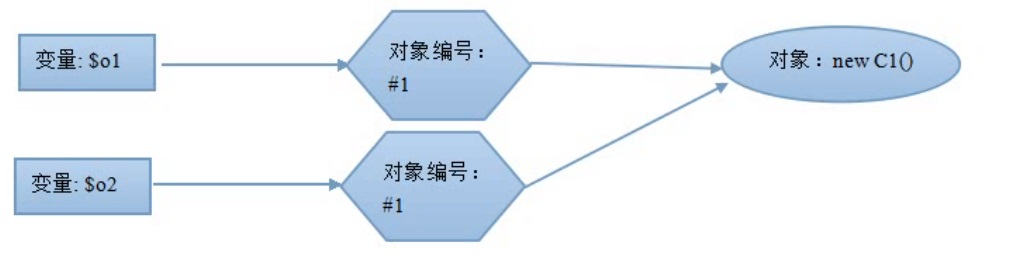
\includegraphics[scale=0.5]{fuzhi}
				\caption{对象赋值}
			\end{figure}
			
			\begin{lstlisting}
	//对象的引用类型传递:
	$o3 = new C1();
	$o4 = &$o3;
	$o3->p1 = 2;
	echo "o3->p1={$o3->p1},o4->p1 = {$o4->p1}";  //o3->p1=2,o4->p1 = 2
			\end{lstlisting}
			对象引用拷贝内存效果如下:
			
			\begin{figure}[H]
				\centering
				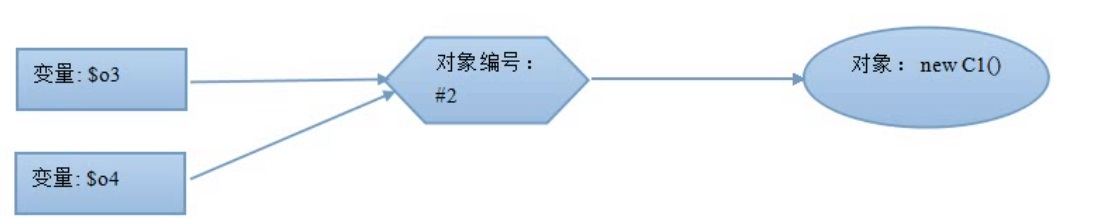
\includegraphics[scale=0.47]{yinyong}
				\caption{对象引用}
			\end{figure}
			
			
		对象编号、克隆、对象模型:\url{https://blog.csdn.net/mizhenxiao/article/details/51909398}
	
	
	\section{闭包}
		闭包的语法很简单,需要注意的关键字就只有use,\textbf{use意思是连接闭包和外界变量}。
		\begin{lstlisting}
	$a =function()use($b) {}
		\end{lstlisting}
		
		
\chapter{开发事宜}
 
 
 
\chapter{工具}
	\section{PhpStorm}
		\url{https://blog.csdn.net/gu_wen_jie/article/details/79136475}
	
	\section{Xdebug}
		配置php.ini \url{https://www.cnblogs.com/LWMLWM/p/8251905.html}
		
		配置phpstorm And webbrows :\url{https://www.cnblogs.com/yxhblogs/p/6598387.html}
 		  			
\end{document} 
 		    